\documentclass{article}

\usepackage{natbib}
\usepackage{hyperref}
\usepackage{graphicx}

\title{Final Report}

\author{
James Atwood and Luis Pineda \\ % alphabetical order
}

\begin{document}
\maketitle

\section{Introduction}
Our project was a submission to the SIGMOD 2014 programming challenge,
where teams are provided with a large (relational) social network
dataset and are asked to implement four queries related to the graph
structure of the data.  Using a relatively simple design and
incremental optimization, we were able to complete our Java
implementation by the April 15th deadline and submit it for
evaluation.  According to the
leaderboards\footnote{\url{http://www.cs.albany.edu/~sigmod14contest/leaders.html} under team name `shparg'},
which provide preliminary results, our entry ranks 22nd out of 32
total submissions.  Unfortunately, the final evaluation on held-out
data will not be released until after this report has been written, so
we can not report our official standing.

The motivation for choosing this project was
twofold; first, there is a large (and quickly increasing) volume of
graph-structured data available today, and second, developing
efficient mechanisms for representing and querying graph data is a
challenging research problem that is currently the subject of
considerable interest in the database community.

\section{Background and Related Work}
\subsection{Challenge Description}

\subsubsection{Data}
We are provided with a relational dataset which describes a social
network.  Example entities include people and places and example
relations include 'knows' and 'lives at'.  Each entity and
relationship is stored as a pipe-delimited file.  Entity files are
named after the entity type (e.g. `person.csv') and contain features.
Relation files are named after the relation they contain
(e.g. `person\_knows\_person.csv') and contain pairs of entities which
have that relation.

\subsubsection{Task}
The task is to return the correct results of a provided set of queries
against the provided data as quickly as possible.  Performance is
first measured by correctness (if any query results are incorrect, a
submission is invalid) followed by runtime (with lower being better).
`Runtime' means the wall-clock time from program initiation to
termination.  Note that subtasks like reading the data into memory or
constructing an index will factor in to the runtime.

\subsubsection{Query types}
There are four types of queries that need to be answered.

\subsubsection{query1(p1, p2, x)}
Given two integer person ids p1 and p2, and another integer x, find
the minimum number of hops between p1 and p2 in the graph induced by
persons who
\begin{enumerate}
\item have made more than x comments in reply to each others'
comments, and
\item know each other.
\end{enumerate}

\subsubsection{query2(k, d)}
Given an integer k and a birthday d, find the k interest tags with the largest range, where the range of an interest tag is defined as the size of the largest connected component in the graph induced by persons who
\begin{enumerate}
\item have that interest,
\item were born on d or later, and
\item know each other.
\end{enumerate}

\subsubsection{query3(k, h, p)}
Given an integer k, an integer maximum hop count h, and a string place
name p, find the top-k similar pairs of persons based on the number of
common interest tags. For each of the k pairs mentioned above, the two
persons must be located in p or study or work at organisations in
p. Furthermore, these two persons must be no more than h hops away
from each other in the graph of people who know each other.

\subsubsection{query4(k, t)}
Given an integer k and a string tag name t, find the k persons who
have the highest closeness centrality values in the graph induced by
persons who
\begin{enumerate}
\item are members of forums that have tag name t, and
\item know each other.
\end{enumerate}


\subsection{Related Work}
Traditionally, research in databases has focused on the relational
model first proposed by Codd \cite{codd1970relational}.  This model
becomes awkward and inefficient when applied to graph data
\cite{rodriguez2011graph}, particularly for queries related to
complex structure (i.e., requiring more than nearest neighbors).  For
an example, please see \cite{he2008graphs} Figures 1 and 2.  More
recent work has proposed other data models and query languages that
more appropriately capture the rich structure evident in graph data;
for instance,
\cite{he2008graphs,sun2012efficient,low2010graphlab} (see
\cite{angles2008survey} for a survey of recent graph database
models).  

%However, much of this work is task oriented; for example, a system
%may optimize for path-related queries at the expense of subgraph
%isomorphism.  For the task at hand, it is unclear which existing
%technologies, if any, provide the best performance for the queries of
%this challenge.

\section{Implementation}
\subsection{Data Representation}
\subsubsection{Embedded Database Design}
Originally, we designed our implementation around the open-source
Neo4j\footnote{\url{http://www.neo4j.org/}} disk-based graph database
system.  We thought this system was appropriate because the queries in
the challenge are largely path-oriented, and it is unlikely that all
of the relevant data will fit in memory.  Neo4j makes use of the
\emph{ADI} index structure \cite[Chapter~6]{IanRobinson:2013ul}
described in \cite{wang2004scalable}, which is designed to facilitate
efficient edge support checking (that is, quickly finding edges) and
adjacent edge checking (that is, quickly finding edges that share a
node).  This index structure seemed well-suited to the task at hand
because it allows a graph on disk to be efficiently queried with
regards to path.

Our implementation of this approach performed very poorly, however.
An implicit assumption of this design was that the high fixed cost of
populating the graph database would be amortized over the large number
of queries against the data.  Instead, we found that the runtime cost 
of reading and indexing the data using Neo4j was prohibitively large,
therefore any potential improvement Neo4j could offer in query performance
would not offset the cost of populating the database.
It seems likely that this undesirable behavior will be found
with other database systems; if fixed setup costs are amortized over
the lifetime of a database system measured in years, the cost of
establishing the database is trivial, so reducing this cost is likely
not a design goal.

\subsubsection{In-Memory Design}
We turned our attention to a simpler key-value approach tailored 
to the SIGMOD challenge dataset. 
Specifically, we indexed nodes and edges via several simple 
in-memory hash tables, one for each type of node or edge 
relevant to the queries. 
This design choice was motivated by an analysis of the provided 
datasets (1k and 10k persons), which suggested that most of the
storage needs are due to node types whose persistence is not needed to 
answer the queries (i.e., comments and forums). With the right 
pre-processing this information is only needed to update information 
only while the database is populated
(e.g., how many comments have persons given to each other).
We suspect that, at least for the 100k persons dataset, the 
relevant part of the graph should fit in the 15Gb of available memory
for the contest (our current implementation uses approx. 800Mb for 
the 10k dataset). Overall, the current memory-based approach 
both reduced the time it took to index the data and improved the speed 
of the queries by orders of magnitude with respect to our initial
Neo4j implementation.

%Accordingly, we propose the following approach.  Our primary data
%abstraction will be an adjacency matrix over the nodes which
%constitute a network.  The nodes will themselves be an interface for
%the data provided by the challenge.  We will be investigating the
%particulars of the implementation of the adjacency matrix and node
%abstractions throughout the project. To be more concrete, a node could
%be an object representing a person, with fields for attributes like
%gender and age.  Or, a node could simply be a pointer to a query which
%retrieves the node's data from disk.  The adjacency matrix could be a
%simple $n$ by $n$ array, where $n$ is the total number of people in
%the dataset.  This adjacency matrix representation scales poorly; we
%will probably need to employ some sparse representation or other
%compression mechanism to maintain this structure in memory, or
%implement some mechanism for managing adjacency matrices that are only
%partially stored in memory, such as the \emph{ADI} structure described
%in \cite{wang2004scalable}. Finally, after developing appropriate
%implementations of the node and matrix abstractions, we will focus on
%developing efficient indexing and graph traversing mechanisms for
%servicing the four types of query that are the subject of the SIGMOD
%challenge.

%Neo4j is a Java system, so our implementation language will be Java.
%We will use the embedded interface of
%Neo4j\footnote{\url{http://docs.neo4j.org/chunked/stable/tutorials-java-embedded.html}}
%in order to construct an indexed graph database from the provided
%data.  This database will be constructed and queried using the Core
%API, which provides the lowest user-level abstractions in the Neo4j
%system, and is generally faster than the higher-level Traversal and
%Cypher APIs \cite[Chapter~6]{IanRobinson:2013ul}.

%The following pseudocode demonstrates how we will use the disk-based
%system to perform the first query, which finds the shortest path
%between two people p1 and p2 who have replied to each other's comments
%at least x times.


%More specifically, our implementation language will be Java.  The
%adjacency matrix representation will initially be implemented as a
%sparse Colt
%matrix \footnote{\url{http://acs.lbl.gov/software/colt/api/cern/colt/matrix/package-summary.html}}.

This memory-based design, implemented in Java, defines data structures for each 
of the relevant entities defined in this database: person, tags, places and 
forums. We also created a specialized edge structure for the person\_knows\_person
relationship that, besides the pointer to the person nodes, also stores
the number of comments that each of the persons have replied to the other (this
is very useful to answer query 1 efficiently). 

Using these structures, our current pipeline is as follows. When the program starts, a
hash table for each edge and node type is populated. In particular, the following hash tables are maintained:

\begin{itemize}
\item A person node table indexed by a 64-bit id number.
\item A tag node table indexed by a 64-bit id number.
\item A place node table indexed by a 64-bit id number.
\item A forum node table indexed by a 64-bit id number. 
\item A commentIDCreatedBypersonID table indexed by a 64-bit id number.
\item A organizationIDLocatedAtPlaceID table indexed by a 64-bit id number.
\item A placeIDLocatedAtPlaceID table indexed by a 64-bit id number.
\item A placesIDWithNames table indexed by a string number specifying the place name. The value is a list of placeIDs that have that name (currently represented as a space separated string of place IDs).
\end{itemize}

These tables are populated by reading files such as person.csv, 
comments.csv, tags.csv, comment\_hasCreator\_person.csv and so forth. 
Each node type stores edges to other nodes whenever there is a relationship
that is useful for answering at least one of the queries. Specifically,
the following edges are stored:

\begin{itemize}
\item A person node stores: a list of edges, one for each known person, a list of pointers to tag nodes the person is interested in, and a list of pointers to place nodes the person is located at.
\item A tag node stores: a list of pointers to interested person nodes and a list of pointers to persons nodes that are members of forums with this tag. 
\item A forum node stores: a list of pointers to tag nodes with the interests of the forum. 
\end{itemize}

%%% LUIS - is this still relevant? %%%
%Additionally, each node type is indexed by properties that are 
%relevant to the queries. Some examples are:
%\begin{itemize}
%\item Indexing tag nodes by id will be useful for performing efficient 
%lookups for query 2.
%\item Indexing organization and place nodes by id will be useful for 
%performing efficient lookups for query 3.
%\item Storing the number of common tags between two persons as part of 
%the KNOWS relationship can be useful for query 3.
%\item Indexing forums by id will be useful for performing efficient lookups 
%for query 4.
%\end{itemize}

\subsection{Query Implementations}

We implement each query as a graph algorithm over the graph defined by
the indexed data.

\subsubsection{Query1} A breadth first search (BFS) of the
person\_knows\_person graph based on the constraint on number of replies
x.  Edges with less than x replies are pruned by the BFS.

\subsubsection{Query2} Add all tags to a priority queue where the order of
the tags is based on the size of the largest connected component of
the induced graph. This uses the list of persons that are interested in the 
tag, and information about the birthday stored by each person node. With
this information, the induced graph is created on-the-fly and the size 
of the connected component is computed using a BFS.
              
\subsubsection{Query3} placesIDWithNames is used to find all placeIDs with
the given name. For each of these places p, we do a linear scan to find 
all persons located at p and add these persons to the induced graph. 
To check if a person is located at p, we use both the 
list of places stored by the person node, but also the table 
placeIDLocatedAtPlaceID to recursively check if any place 
in the induced hierarchy is contained in p. If at least one does, 
the person is added to the induced graph.
              
When all the relevant persons are added to the graph, 
the similarity score of all possible pairs of persons in this
graph is computed and these are added to a priority queue. To speed up
the similarity computation, the list of persons
interested in that tag node is indexed by person id. 
Therefore the similarity between two persons can be computed in 
linear time on the number of interest tags.
              
\subsubsection{Query4} First a linear search is used to find the tag with
the given name. Then the induced graph of persons that are member of
forums with this tag is created, using the list stored by each tag node.
               
On the induced graph the centrality score of each person is computed
by using a BFS. Every time a node is expanding during the BFS, the
algorithm checks if the best possible centrality this person can
achieve is smaller than the k-th best centrality seen so far. If it
is, the BFS is stopped.

\section{Results}
\begin{figure}
  \centering
  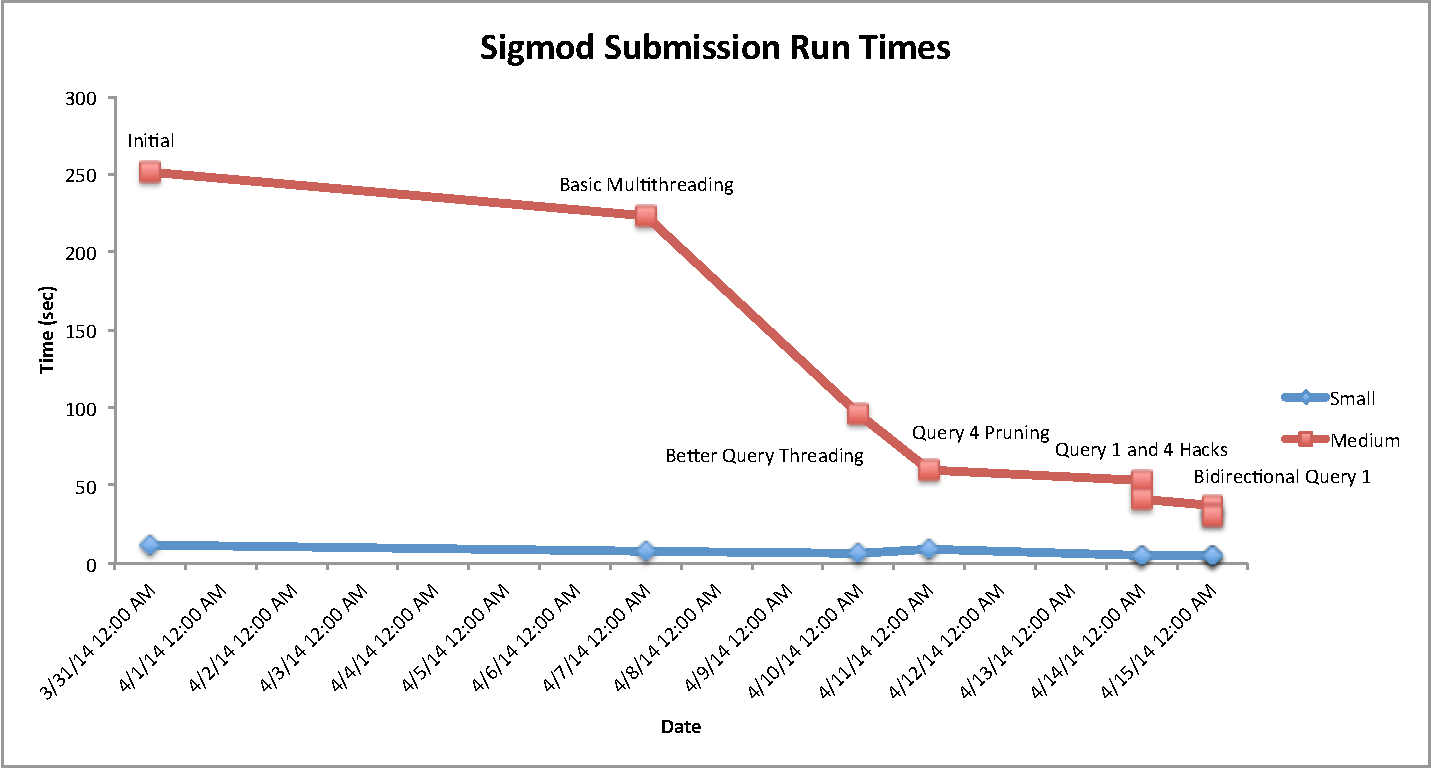
\includegraphics[scale=0.5]{img/results.pdf}
  \label{fig:results}
  \caption{Evolution of the performance of our implementation on the
    SIGMOD system.  The horizontal axis gives the date of the
    submission and while the vertical axis shows the runtime as
    reported by the submission system.  Each submission is annotated
    with the optimizations that were introduced with it.  `Medium'
    indicates the dataset with 10,000 people and `Small' the dataset
    with 1,000 people.}
\end{figure}

Our implementation's performance is shown in Figure \ref{fig:results}.  All times were provided by the SIGMOD
submission system.  According to the challenge description\footnote{\url{http://www.cs.albany.edu/~sigmod14contest/task.html}}, performance was measured on a server with the following specification:
\begin{itemize}
\item Processors: Two 2.67 GHz Intel Xeon E5430 (4 cores each, 8 cores total)
\item Main Memory: 15 GB
\item OS: Red Hat Enterprise Linux Server 6.5 (Santiago) 
\item Java: JDK 1.7.0
\end{itemize}

%Overall, we are currently ahead of the schedule we proposed; all queries are implemented and we have submitted an implementation to SIGMOD.  Our results can be seen on the
%leaderboard\footnote{\url{http://www.cs.albany.edu/~sigmod14contest/leaders.html}} under team name `shparg'.
%
%Progress on Project Milestones:
%\begin{itemize}
%\item Early March: Download datasets; setup Neo4j library;
%  design of pipeline; implementation of queries 1 and 2 on small test dataset. \textbf{DONE}
%\item March 20th: Implementation of queries 3 and 4 on small test dataset. \textbf{DONE}
%\item April 1st: Submit midterm report. \textbf{DONE}
%\item April 8th:  Run experiments with the larger dataset. \textbf{DONE} \\Refine the implementation to address scalability issues.
%\item April 15th: Submit system to SIGMOD if we have a competitive entry. \textbf{DONE}
%\item April 29th: Present results to class.
%\item May 8th: Final report.
%\end{itemize}
%
%We will devote our remaining time to improving performance and
%addressing scalability issues.  Our main idea is to use a disk-based
%extensible hash to index the nodes and edges over the original
%(unsorted) heap files\footnote{which implies we will be using
%  Alternative 3 for the index data entries.} so that we may avoid
%loading the entire dataset into memory.  This index is appropriate
%because we are only concerned with equality searches. 
%
%Additionally, we are going to add multi-threading capabilities to our
%system, in order to take advantage of the 8 cores available on the SIGMOD computers. 
%Since all queries can be answered independently are no data is added after 
%the initial database population, implementing multiple threads should 
%be straightforward.

\bibliographystyle{abbrv}
\bibliography{final}

\end{document}
